\documentclass[12pt,english]{article}
\usepackage[T1]{fontenc}
\usepackage[latin9]{inputenc}
\usepackage{graphicx}
\usepackage{epsfig}

\makeatletter

%%%%%%%%%%%%%%%%%%%%%%%%%%%%%% LyX specific LaTeX commands.
%% Because html converters don't know tabularnewline
\providecommand{\tabularnewline}{\\}

%%%%%%%%%%%%%%%%%%%%%%%%%%%%%% User specified LaTeX commands.
%%%%%%%%%%%%%%%%%%%%%%%%%%%%%%%%%%%%%%%%%%%%%%%%%%%%%%%%%%%%%%%%%%%%%
% PREAMBLE
%%%%%%%%%%%%%%%%%%%%%%%%%%%%%%%%%%%%%%%%%%%%%%%%%%%%%%%%%%%%%%%%%%%%%
% The following two commands will generate a PDF that follows all the
%requirements for submission
% and peer review.  Uncomment these commands to generate this output (and
%comment out the two lines below.)
% DOUBLE SPACE VERSION FOR SUBMISSION TO THE AMS
\usepackage{ametsoc}% The following two commands will generate a single space,
%double column paper that closely
% matches an AMS journal page.  Uncomment these commands to generate this output
%(and comment
% out the two lines above. FOR AUTHOR USE ONLY. PAPERS SUBMITTED IN THIS FORMAT
%WILL BE RETURNED
% TO THE AUTHOR for submission with the correct formatting.
% TWO COLUMN JOURNAL PAGE LAYOUT FOR AUTHOR USE ONLY
%%%%\documentclass[10pt]{article}
%%%%\usepackage{ametsoc2col}
%%%%%%%%%%%%%%%%%%%%%%%%%%%%%%%%%%%%%%%%%%%%%%%%%%%%%%%%%%%%%%%%%%%%%
% ABSTRACT
% Enter your Abstract here
%%%%%%%%%%%%%%%%%%%%%%%%%%%%%%%%%%%%%%%%%%%%%%%%%%%%%%%%%%%%%%%%%%%%%
\newcommand{\myabstract}{Enter abstract here.}

\makeatother

\usepackage{babel}

\begin{document}
%%%%%%%%%%%%%%%%%%%%%%%%%%%%%%%%%%%%%%%%%%%%%%%%%%%%%%%%%%%%%%%%%%%%%
% TITLE
% Enter your TITLE here
%%%%%%%%%%%%%%%%%%%%%%%%%%%%%%%%%%%%%%%%%%%%%%%%%%%%%%%%%%%%%%%%%%%%%



\title{\textbf{\large {The Great Lakes Wave Model at NCEP/NOAA: }\\
\textbf{\large{} Implementation, General Features and Future Developments}}}

\maketitle
% Author names, with corresponding author information. 
% [Update and move the \thanks{...} block as appropriate.]

\author{\textsc{Author One}
                                \thanks{\textit{Corresponding author address:}
                                Rua Sobe e Desce, Number 000
                                \newline{E-mail:
someone@noaa.gov}}\quad\textsc{Author Two}\\
\textit{\footnotesize{Somewhere, over the rainbow}}
\and
\centerline{\textsc{Extra Author}}\\% Add additional authors, different
insitution
\centerline{\textit{\footnotesize{Affiliation, City, State/Province, Country}}}
}



% Formatting done here...Authors should skip over this.  See above for abstract.
\ifthenelse{\boolean{dc}} { \twocolumn[
\begin{@twocolumnfalse}
\amstitle

\begin{center}
\begin{minipage}{13.0cm}
\begin{abstract}
	\myabstract
	\newline
	\begin{center}
		\rule{38mm}{0.2mm}
	\end{center}
\end{abstract}
\end{minipage}
\end{center}
\end{@twocolumnfalse}
] } { \amstitle 
\begin{abstract}
\myabstract 
\end{abstract}
} %%%%%%%%%%%%%%%%%%%%%%%%%%%%%%%%%%%%%%%%%%%%%%%%%%%%%%%%%%%%%%%%%%%%%
% MAIN BODY OF PAPER
%%%%%%%%%%%%%%%%%%%%%%%%%%%%%%%%%%%%%%%%%%%%%%%%%%%%%%%%%%%%%%%%%%%%%

\section{~Introduction}
\vssub
\subsection{~About this manual}
\vssub

This is the user manual and system documentation of version \WWver\ of the
 third-generation wind-wave modeling framework \ww. This underlying model has
 been developed at the Marine Modeling and Analysis Branch (MMAB) of the
 Environmental Modeling Center (EMC) of the National Centers for Environmental
 Prediction (NCEP). It is based on WAVEWATCH~I and WAVEWATCH~II as developed
 at Delft University of Technology, and NASA Goddard Space Flight Center,
 respectively. \ws\ differs from its predecessors in all major aspects; i.e.,
 governing equations, program structure, numerical and physical
 approaches. %\wt\ is a trademark of the United States government.

This manual describes the governing equations, numerical approaches,
compilation, and running of \ws. The format of a combined user manual and
system documentation has been chosen, to give users the necessary background
to include new physical and numerical approaches in the framework according to
their own specifications.  This approach became more important, as \ws\
developed into a wave modeling framework. By design, a user can apply his or
her numerical or physical approaches, and thus develop a new wave model based
on the \ws\ framework. In such an approach, optimization, parallelization,
nesting, input and output service programs from the framework can be easily
shared between actual models.  Whereas this document is intended to be
complete and self-contained, this is not the case for all elements in the
system documentation. For additional system details, reference is made to the
source code, which is fully documented. Note that a best practices guide for
code development for \ws\ is now available \citep{tol:MMAB09b}.

The governing equations and numerical approaches used in this model are
described in chapters~\ref{chapt:eq} and \ref{chapt:num}. Running the model is
described in chapter~\ref{chapt:run}. Installing \ws\ is described in
chapter~\ref{chapt:impl}. Finally, a short system documentation is given in
chapter~\ref{chapt:sys}. A thorough knowledge of \ws\ can be obtained by
following chapters~\ref{chapt:eq} through \ref{chapt:impl}. A shortcut is to
first install the model (chapter~\ref{chapt:impl}), and then successively
modify input files in example runs (chapter~\ref{chapt:run}).

\vspace{\baselineskip} 
\pb
\noindent 
The present model version (\WWver) is a developmental version based on the
last official model release (version 3.14). Since the latter release the
following modifications have been made:

\begin{list}{$\bullet$}{\rightmargin 5mm \parsep 0mm \itemsep 0mm}

\item
The code is now maintained using subversion \citep{bk:CSea06}. For
co-developers, a script is available to install \ws\ directly from the
repository at NCEP \citep[see][]{tol:MMAB09b} (model version 3.14/4.00).

\item
Slot for new grids (model version 4.01)

\item
Slot for new grids (model version 4.02)

\item
\ldots (model version 4.03)

\end{list}

\vspace{\baselineskip} \noindent 
A note of caution. \ww\ includes wave-current interactions. The implementation
of these interactions has only been tested in idealized test cases. Only
limited tests in realistic conditions have been performed.

\vspace{\baselineskip} \noindent 
Up to date information on this model can be found (including bugs and bug
fixes) on the \ww\ web page, and comments, questions and suggestions should be
directed to the corresponding E-mail address

\begin{center}
http://polar.ncep.noaa.gov/waves/wavewatch \\
NCEP.EMC.wavewatch@NOAA.gov
\end{center}

\noindent
We will redirect questions regarding contributions from outside NCEP to the
respective authors of the codes.


\vssub
\subsection{~Licensing terms}
\vssub

Starting with model version 3.14, \ww\ is distributed under the following
licensing terms:

\vspace \baselineskip \noindent
\centerline{
\rule[1mm]{47mm}{.5mm} {\rm start of licensing terms}
\rule[1mm]{47mm}{.5mm}}

\vspace \baselineskip \noindent 
Software, as understood herein, shall be broadly interpreted as being
inclusive of algorithms, source code, object code, data bases and related
documentation, all of which shall be furnished free of charge to the Licensee.

Corrections, upgrades or enhancements may be furnished and, if furnished,
shall also be furnished to the Licensee without charge. NOAA, however, is not
required to develop or furnish such corrections, upgrades or enhancements.

NOAA's software, whether that initially furnished or corrections or upgrades,
are furnished “as is.” NOAA furnishes its software without any warranty
whatsoever and is not responsible for any direct, indirect or consequential
damages that may be incurred by the Licensee.  Warranties of merchantability,
fitness for any particular purpose, title, and non-infringement, are
specifically negated.

The Licensee is not required to develop any software related to the licensed
software.  However, in the event that the Licensee does so, the Licensee is
required to offer same to NOAA for inclusion under the instant licensing terms
with NOAA's licensed software along with documentation regarding its
principles, use and its advantages.  This includes changes to the wave model
proper including numerical and physical approaches to wave modeling, and
boundary layer parameterizations embedded in the wave model The Licensee is
encouraged but not obligated to provide pre-and post processing tools for
model input and output.  The software required to be offered shall not include
additional models to which the wave model may be coupled, such as oceanic or
atmospheric circulation models. The software provided by the Licensee shall be
consistent with the latest model version available to the Licensee, and
interface routines to the software provided shall conform to programming
standards as outlined in the model documentation. The software offered to NOAA
shall be offered as is, without any warranties whatsoever and without any
liability for damages whatsoever.  NOAA shall not be required to include a
Licensee's software as part of its software.  Licensee's offered software
shall not include software developed by others.

A Licensee may reproduce sufficient software to satisfy its needs.  All copies
shall bear the name of the software with any version number as well as
replicas of any applied copyright notice, trademark notice, other notices and
credit lines.  Additionally, if the copies have been modified, e.g. with
deletions or additions, this shall be so stated and identified.

All of Licensee's employees who have a need to use the software may have
access to the software but only after reading the instant license and stating,
in writing, that they have read and understood the license and have agreed to
its terms.  Licensee is responsible for employing reasonable efforts to assure
that only those of its employees that should have access to the software, in
fact, have access.

The Licensee may use the software for any purpose relating to sea state
prediction.

No disclosure of any portion of the software, whether by means of a media or
verbally, may be made to any third party by the Licensee or the Licensee's
employees

The Licensee is responsible for compliance with any applicable export or
import control laws of the United States.

\vspace \baselineskip \noindent
\centerline{
\rule[1mm]{48mm}{.5mm} {\rm end of licensing terms}
\rule[1mm]{48mm}{.5mm}}

\vspace \baselineskip \noindent
The software will be distributed through our web site after the Licensee has
agreed to the license terms.


\vssub
\subsection{~Copyrights and trademarks}
\vssub

\ww\ \copyright\ 2009 National Weather Service, National Oceanic and
Atmospheric Administration.  All rights reserved. \ww\ is a trademark of the
National Weather Service. No unauthorized use without permission.

\vssub
\subsection{~The development group}
\vssub

Even in its original development, when I was working on the code mostly on my
own on the development of \ww, many have contributed to the success of the
model. With the expansion of physical and numerical parameterizations
available, the list of contributors to this model is growing. I would like to
recognize the following contributors as the development group (in alphabetic
order) :

\begin{list}{\ldots}{ }
\item [Henrique Alves] (Metocean Engineers, Australia) \\
Support of code development while at NCEP, shallow water physics packages.
\item [Fabrice Ardhuin] (Service Hydrographique et Oc\'{e}anographique de la
Marine, France) \\
Various  physics packages.
\item [Nico Booij] (Delft University of Technology, The Netherlands) \\
Original design of source code pre-processor ({\code w3adc}), basic method of
documentation and other programming habits. Spatially varying wavenumber grid.
\item [Dmitry V. Chalikov] (ESSIC, Univ. of Maryland, USA) \\ Co-author of the
\cite{tol:JPO96} input and dissipation parameterizations and source code.
\item [Arun Chawla](Science Applications International Corporation, USA) \\
Support of code development at NCEP, GRIB packing, automated grid generation
software \citep{tol:MMAB07a, tol:OMOD08a}.
%\item [Vladimir Krasnopolsky] (Science Applications International Corporation,
%  USA) \\
%Neural Network nonlinear interaction approaches.
\item [Barbara Tracy] (US Army Corps of Engineers, ERDC-CHL, USA) \\
Spectral partitioning
\item [Gerbrant Ph. van Vledder] (Alkyon Hydraulic Consultancy \& Research,
NL) \\ 
Webb-Resio-Tracy exact nonlinear interaction routines, as well as some of the
original service routines.
\end{list}


\vssub
\subsection{~Acknowledgments}
\vssub

The development of \ww\ has been an ongoing process for well over a
decade. The development of WAVEWATCH I was entirely funded through my
Ph.D. work at Delft University. The development of WAVEWATCH II has been
funded entirely through my position as a National Research Council Resident
Research Associate at NASA, Goddard Space Flight Center. The initial
development of WAVEWATCH III version 1.18 was entirely funded by NOAA/NCEP,
with most funding provided by the NOAA High Performance Computing and
Communication (HPCC) office. Developments of version 2.22 have been funded
similarly through NOAA/NCEP. Since then, funding is provided by NCEP, but also
by many partners outside NCEP. Much of the work at NCEP has been performed
under contract by Science Applications International Corporation (SAIC).
Special thanks are due to to The Office of Naval Research (ONR), for the
funding of many upcoming model upgrades.

I would finally like to thank all users who have reported errors and glitches,
or have made suggestions for improvements, particularly those who have
beta-tested this and previous model release.

%\bpage


\section{Local wave climate}

(to be written, hopefully by David Schwab or Paul Liu??)


\section{Previous Great Lakes Wave Modeling Efforts}

Forecasts and hindcasts of wind waves at the Great Lakes, made with numerical
prediction schemes or models, have been generated since the early 1970's. Since
then, the techniques applied to wave hindcasting have followed more closely the
latest trends and techniques made available throughout time. Wave forecasting,
however, until recently has favoured older modelling approaches based on
parametric models, that are still applicable in the region due to the
predominance of wave climates associated with short fetches and local wind
generation. 

The need for more detailed description of complex wave generation scenarios, and
shallow-water wave propagation, has provided a push towards upgrading wave
forecasting models in the region. In this section we provide a brief, general
history of both wind-wave hindcasting and forecasting in the Great Lakes. 


\subsection{Hindcasts}

The first long-term Great Lakes wave hindcast product generated using a
numerical scheme for computing waves from wind data is presented in
\cite{resvin76}. The technique was based on overlake wind data estimated from
overland measurements and ship anemometers. These early hindcasts covered a
69-year period (1907-1975), and were a useful source of wave data for
engineering applications in the Great Lakes during the late 1970's and 1980's.

With the advent of a two-dimensional model for wave simulation within the Great
Lakes, the Ontario Ministry of Natural Resources funded in the mid-1980's the
development of a new wave climate database, with the latest available
technology, as part of its shoreline management plan. The approach consisted of
using the \cite{schwet84a} wave model, forced with gridded overlake winds
derived from overland measurements via an estimation technique described in
\cite{philirb78}. Results were assembled onto wave hindcast databases for
individual basins within the Great Lakes system.

In a series of Wave Information Studies (WIS), the USACE has been generating and
constantly upgrading more recent wave hindcast databases in several oceanic
basis, and in major inland water bodies such as the Great Lakes. Fot the latter,
the WIS program has provided two distinct data streams. In the first, the wave
model WISWAVE was run for a 32-year period (1956-1987) over a 10-mile-resolution
grid, using gridded winds derived from land stations via adjustments for the
transition between land-water boundary layers, stability and measurement height.
This first WIS database was later extended for the period 1988-1997, using
improved wind estimates developed in partnership with GLERL that included buoy
measurements available in the Great Lakes since early 1980's. A general
description is provided in \cite{linres01}.

USACE's WIS has recently upgraded the Great Lakes wind-wave hindcast database
with higher-resolution hindcasts produced for Lake Ontario. Wave simulations
were made for a 40-year period (1961-2000), using an upgraded version of WISWAVE
model baptized WAVAD. The hindcasts were generated using a 3km grid covering
Lake Ontario, with wind fields derived from land-based meteorological stations
and buoys and ice concentrations assembled from databases developed by
\cite{asset83}, for the first 14 years, and at GLERL for the remaining period. A
full description of the Lake Ontario hindcasts, which have been made available
since 2003, is provided in USACE's Field Research Facility website
\citep{wisweb}.

\subsection{Forecasts}

A first wave guidance product for the Great Lakes based on numerical schemes was
implemented in 1974 by the US National Weather Service (henceforth NWS), which
consisted of forecasts of sea state extending out to 36 hours, at 12-h
intervals. These early wave forecasts were computed using an automated numerical
scheme developed by \cite{pore74}, based on an adaptation of the method by
\cite{bret70}, both cited in \cite{burrdal97}. 

In response to requests made by the forecasting community to expand the wave
forecasts generated by the NWS in the 1970's, which were limited to 64 fixed
locations, the Great Lakes Environmental Research Laboratory (GLERL) developed a
two-dimensional wind-wave model, which was later implemented for operational
forecasting in the region. The deployed model was a first-generation wind-wave
model, solving a local momentum balance equation over a grid with resolution at
5 km or 10 km for different lakes. Ice coverage is ignored. Detailed history and
description of the GLERL wave model are provided in \cite{schwet84a,schwet84b},
whereas the initial validation that led to its operational implementation are
reported in \cite{liuet84}. 

As pointed out by \cite{liuet84}, the implemented model at GLERL was ``not
without drawbacks. It is purely a wind-wave prediction model and has no
provision for swell propagation at present. [...] In addition, the model is for
deep-water waves and the results may not be accurate for shallow-water waves''.
The concerns expressed by \cite{liuet84} were the central motivation pushing
NOAA/NCEP efforts towards implementing a state-of-the-art, third-generation
spectral wind-wave model, where not only swell propagation but also
shallow-water and nonlinear processes may be represented for a full
two-dimensional wave energy-density spectrum. 

A first implementation of the WAVEWATCH III model at the Great Lakes region was
made in an independent effort by the NWS Weather Forecast Office at Marquette,
Illinois (Thomas Hultquist, personal communication, 2004). Several case studies
were performed, using winds generated with the RAMS model. Results were
promising, and established loosely the feasibility of running WAVEWATCH III
operationally for wind-wave forecasting at the Great Lakes.


\section{The Great Lakes wave model at NOAA/NCEP}

The WAVEWATCH III model has been implemented operationally by NOAA/NCEP for most
major weather forecast guidance areas in the world under USA jurisdiction since
2000. With the objective to extend this standard NOAA/NCEP wind-wave forecasting
guidance approach to the Great Lakes, the Environmental Modeling Center (EMC) at
NOAA/NCEP launched, in 2004, a formal project envisaging the operational
implementation of WAVEWATCH III in the region within a 2-year time frame. 

The initial plan included using the WAVEWATCH III model with wind fields derived
from the ETA model. Ice concentrations were to be included int he system,
provided by operational analyses made at the NOAA/NCEP. Also planned was the
inclusion of dynamically updated mean water levels on a seasonal time scale.
WAVEWATCH III was to be implemented in a single grid encompassing the five major
lakes that integrate the Great Lakes system -- Erie, Huron, Michigan, Ontario
and Superior.

\subsection{Initial implementation}

The initial implementation of a Great Lakes model based on NOAA/NCEP's WAVEWATCH
III code (henceforth the GLW model), begun in late 2004. During the first three
quarters of 2005, a wave forecasting system
using WAVEWATCH III was developed and tested, and by late 2005, a
pre-operational version of the GLW model was deployed. In June 2006, an
experimental web site made available
the four-times daily GLW forecasts for public access. In August 2006,
the experimental GLW system was made operational within the US National
Weather Service suite of numerical weather prediction models. 

In this section, a brief overview of the work undertaken in this first, initial
implementation period is provided.

\subsubsection{Spectral resolution}

In the major oceanic basins, waves can develop over long fetches and propagate
long distances, originating wave-energy spectra that may contain significant
amounts of energy in very low frequencies (eg, of the order of 0.04Hz).
Therefore, typical wind-wavel models use discrete energy spectra with
frequencies ranging from 0.04Hz up to 0.5Hz. The confined nature of the lakes
geographical features limits the fetch size and propagation distances to a point
that the development of lower frequencies is significantly constrained, relative
to the open ocean. In the absence of previous records in the literature about
the occurrence of low fequency wind-waves in the region, a brief investigation
was made using the National Data Buoy Center (NDBC) buoy measurements archives,
with the objective of determining the most appropriate spectral ranges to be
used in an operational implementation of WAVEWATCH III in the Great Lakes.

A compilation of ``spectral climatologies'' was made at all available NDBC
buoys. Due to the fact many NDBC buoys are removed during the winter months to
avoid damadge from heavy icing, it was assumed that the NDBC data may lack
information on spectral properties of more extreme waves generated by intense
winter storms. Such gap was filled via running WAVEWATCH III with extreme
sustained winds over the longest possible fetches found in the lakes region. As
a consequence of merging the NDBC climatology with the extreme-forcing model
results, it was decided that a discrete spectrum with 29 frequencies ranging
from 0.05 Hz to 0.72 Hz, would be physically appropriate and computationally
feasible.

\subsubsection{Spatial resolution and bathymetric grids}

Land boundary constraints in the Great Lakes wave generation basins make
coastline resolution and issue as important as wind resolution in building a
forecasting system for the region. Coastline shape determines fetch geometry,
and coastline features are important to compute properly wave blocking. Other
strong constraint that had to be considered in defining model resolutions was
the available computer time for operational forecasting at, initially, a time
window of up to 84h (eg, a total of 90h model run considering a 6h hindcast
window). Taken altogether, wind resolution, land boundary geometries and
available operational computing time, led to a compromise spatial wave model
grid resolution at 0.035$^\circ$ in longitude, by 0.05$^{\circ}$ in latitude.

The bathymetric grid for the new WAVEWATCH III system at the Great Lakes was
initially designed using depth obtained directly from GLERL's operational wave
model. Resolution of the originating grids were at X by X, which resulted in a
degraded bathymetric database considering the target resolutions. To reduce this
deficiency, higher resolution bathymetry was obtained for lakes X and Y, which
were kindly made available by. Grids generated via bi-linear interpolation of
these provided higher-resolution databases were used for pre-operational tests,
which indicated they were fit for operational purposes, and are still used in
the current forecasting system at NOAA/NCEP. Figure \ref{fig:bathy} illustrates
the Great Lakes bathymetry currently used operationally.

\subsubsection{Wind fields}

Wind fields were initially obtained from the ETA model, which was the source of
operational forecasts for the continental United States are between X and Y.
Soon after the Great Lakes wave model implementation efforts were started,
NOAA/NCEP shifted its atmospheric forecasting system to the NAM model. The
latter is currently the basis of the operational system that provides wind
fields for the Great Lakes wave model. Resolutions of the NAM model at the time
of implementation of the new wave modeling system were at 1/12$^{\circ}$. 

Validation of NAM winds was made against the following NDBC and Environment
Canada
buoys: 5001, 45007, 45137, 45154,
PILM4 45002, 45008, 45139, 45159, ROAM4 45003, 45012, 45142, 45160, SGNW3 45004,
45132, 45143, DBLN6, STDM4 45005, 45135, 45147, DISW3 45006, 45136, 45149 and
LSCM4. Detailed information about these stations may be obtained directly at the
NDBC website (http://ndbc.noaa.gov). Results revealed two major 
sources of significant biases to the surface wind
fields available to forcibng the wave model: a generalized bias, 
which varied with classes of wind speeds, and a bias associated with
wind direction and distance to shore.

Assessment of model performance at selected buoy location was made both at the
individual and the bulk levels. Individual assessments included investigating
histograms of wind direction, scatter-plots of wind speed at all directions and
at four quadrants (0-90, 90-180, 180-270 and 270-360) and associated linear
regression lines and linear regression lines forced through zero. An example of
the typical outputs used in these individual assessments is provided in Figure
\ref{fig:4q45005}.

\begin{figure}[h!]
 \centering
 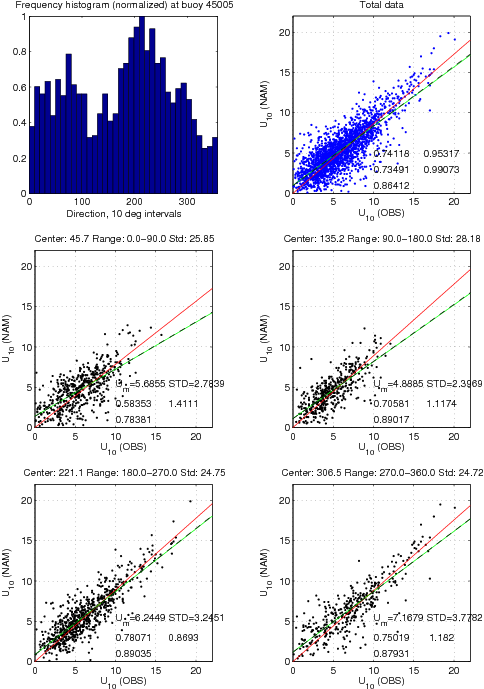
\includegraphics{./figures/fig_45005_4q.png}
 % fig_45005_4q.ps: 490x699 pixel, 72dpi, 17.29x24.66 cm, bb=0 0 490 699
 \label{fig:4q45005}
\end{figure}
 
Bulk assessment of NAM data indicated that surface winds were underestimated at
low wind speeds smaller than 5 m/s, underestimated by 10\% to 20\% in the 5m/s
to 15m/s range and in good agreement for larger intensities. Figure
\ref{fig:nambulk} illustrates the results. Analyses of individual locations
indicated a similar trend, but also revealed the existence of a consistently
higher bias of surface winds near the coastlines. The problem sparkled an
investigation about land-sea boundary issues in the NAM simulations, which will
be explored in more details below. Figure \ref{fig:namshorebias} summarizes the
percentage biases found at selected locations, as a function of distance to the
shoreline.

\begin{figure}[h!]
 \centering
 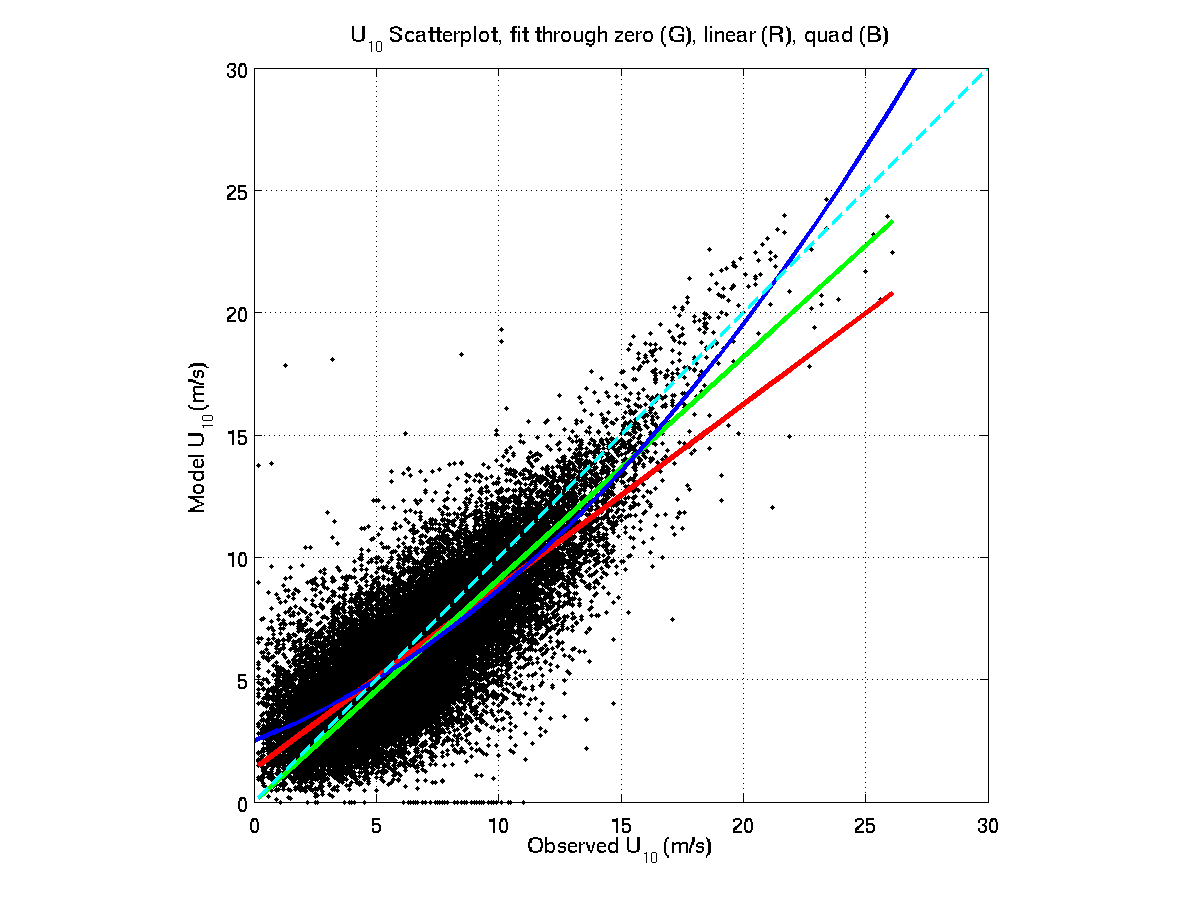
\includegraphics{./figures/fig_nambulk.png}
 % fig_nambulk.eps: 0x0 pixel, 300dpi, 0.00x0.00 cm, bb=
 \label{fig:nambulk}
\end{figure}

\begin{figure}[h!]
 \centering
 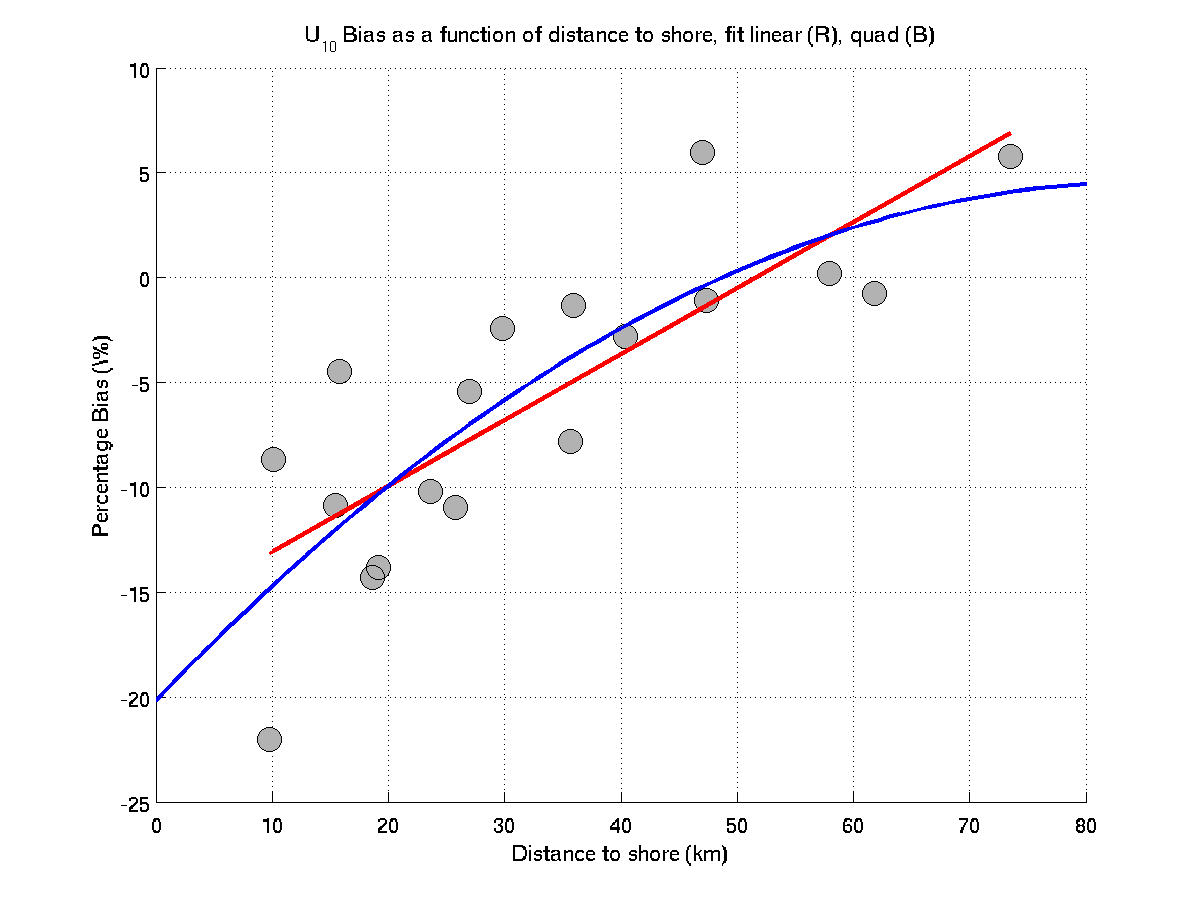
\includegraphics{./figures/fig_namshorebias.png}
 % fig_namshorebias.eps: 0x0 pixel, 300dpi, 0.00x0.00 cm, bb=
 \label{fig:namshorebias}
\end{figure}

Investigations for developing separate strategies for correcting bulk and
distance-to-shoreline biases were initiated independently. Bulk bias correction
was attempted using the average slope of linear regression lines through zero.
Validation statistics indicated that model results were generally insensitive to
the bulk correction, so that a decision was made to go ahead with a future
operational implementation without a bulk surface wind correction component.

A distance-to-shoreline correction scheme was initially envisaged using an
empirical fetch-dependent formula derived from error statistics for NAM surface
winds relative to buoy data. Error maps at selected locations as a function of
wind speed and direction were generated, an illustration of such maps is
provided for station DBLN6 in Figure \ref{fig:nambins}. Global statistics were
then derived from such error maps in an attempt to define a generalized
relationship between wind speed biases and wind fetch geometry. 

\begin{figure}[h!]
 \centering
 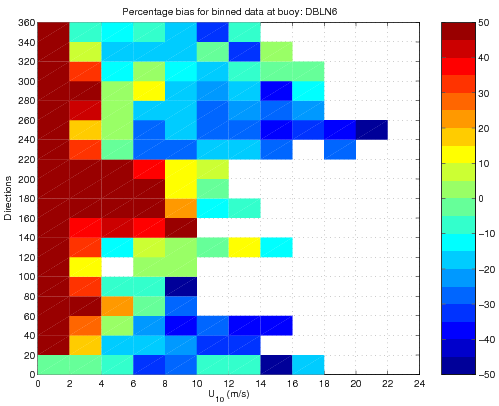
\includegraphics{./figures/fig_DBLN6_bins.png}
 % fig_DBLN6_bins.png: 499x406 pixel, 72dpi, 17.60x14.32 cm, bb=0 0 499 406
 \label{fig:nambins}
\end{figure}

Obtaining generally consistent relationships for correcting wind speeds, based
on fetch geometry, were encouraging. However, the relatively small number of
buoys available in the Great Lakes region, and the fact they are removed during
winter months, limited the reliability of the derived relationships.
Furthermore, as will be explored in more details below, the WAVEWATCH III model
physics, developed mostly for deep-water applications, showed significant
limitations in simulating waves in short-fetch scenarios. 

As a consequence, it was decided that an initial operational implementation of
WAVEWATCH III in the Great Lakes would not include a distance-to-shoreline
correction scheme, until the wave model package included more appropriate
physics to deal with short-fetch wave generation. The correction scheme would be
built based on results summarized above, but would also consider other empirical
and theoretical ideas on land-sea boundary transitions suffered by surface wind
fields. The latter is further discussed below.

\subsubsection{Ice coverage}

The initial operational implementation of the GLW model uses ice concentrations
obtained directly from the NAM atmospheric model data. The latter has a land-sea
mask which is slightly different to that used in the GLW grid, so that
corrections are made. Such correction also account for inconsistencies in ice
coverage close to land boundaries when offshore ice is present at a distance
smaller than a given threshold. If the latter is true, then the ice
concentrations are extended from offshore to the land boundary. The next phases
of upgrades to the GLW system will include high-resolution ice products which
have become available within NOAA/NCEP's operational system.

\subsubsection{Water levels}

Water levels in the Great Lakes show seasonal and longer-term fluctuations. In
both cases, the order of magnitude of water level fluctuations is at 2m. Such
changes may cause differences in wave propagation patterns in nearshore areas.
An assessment of how much water levels affect wave simulations in the region has
been planned, so that future upgrades to the GLW model may include a slow,
seasonal water level variation based on time-averaged gage data for each
individual lake.



\subsection{Deployment of the operational GLW model}

\subsubsection{Initial performance assessments}

\subsection{Upgrades to the operational implementation}

\subsubsection{Performance of current operational forecasts}

\section{Recent research and developments}

\section{Concluding remarks}

\begin{acknowledgment} Start acknowledgments here. \end{acknowledgment}

% Create a bibliography directory and place your .bib file there.
\ifthenelse{\boolean{dc}} {} {\clearpage{}} \bibliographystyle{./ametsoc}
\bibliographystyle{ametsoc}
\bibliography{bibliography/references}


%%%%%%%%%%%%%%%%%%%%%%%%%%%%%%%%%%%%%%%%%%%%%%%%%%%%%%%%%%%%%%%%%%%%%
% FIGURES
%%%%%%%%%%%%%%%%%%%%%%%%%%%%%%%%%%%%%%%%%%%%%%%%%%%%%%%%%%%%%%%%%%%%%
%
%\begin{figure}[t]
% 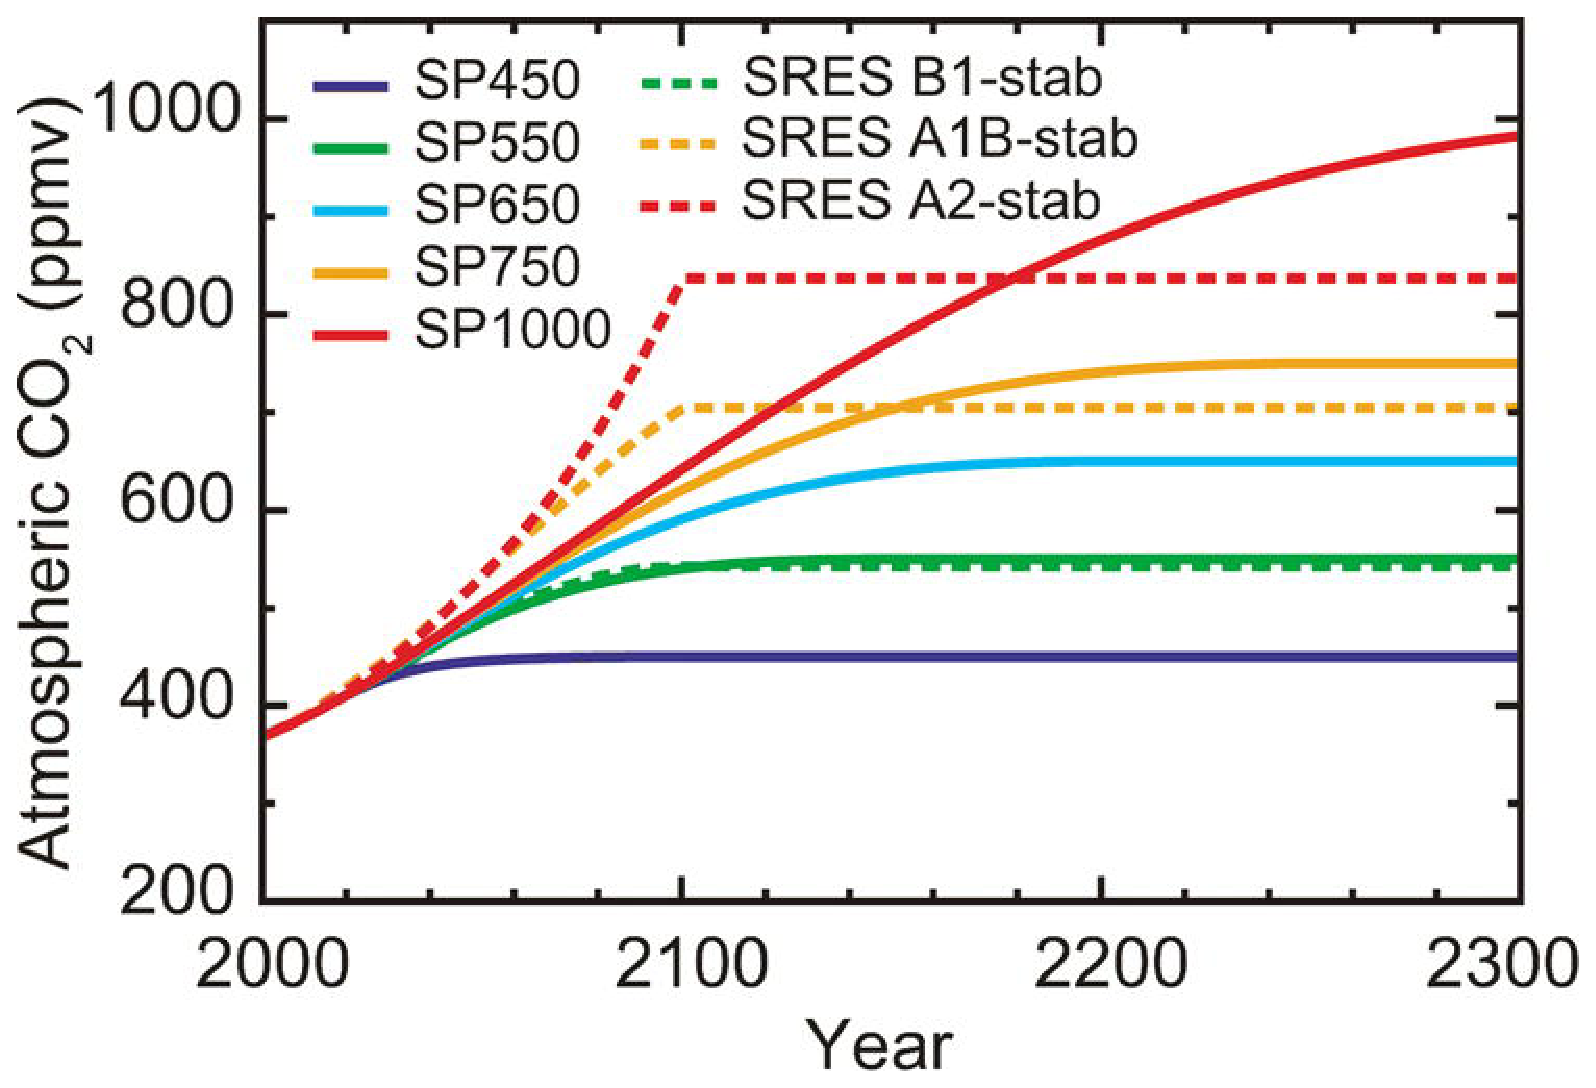
\includegraphics[width=19pc]{figures/figure01}\\
% \caption{Enter the caption for your figure here. Repeat as necessary for each
%of your figures. Create a figures directory and place all figures
%in that directory. Figure from Houghton et al. (2001).}


%\noindent \label{f1} 
%\end{figure}


%%%%%%%%%%%%%%%%%%%%%%%%%%%%%%%%%%%%%%%%%%%%%%%%%%%%%%%%%%%%%%%%%%%%%
% TABLES
%%%%%%%%%%%%%%%%%%%%%%%%%%%%%%%%%%%%%%%%%%%%%%%%%%%%%%%%%%%%%%%%%%%%%
%
%\begin{table}[t]
% \caption{This is a sample table caption and table layout. Enter as many tables
%as necessary at the end of your manuscript. Table from Lorenz (1963).}

%\label{t1} 

%\centering{}\begin{tabular}{ccccrrcrc}
%\hline 
%$N$  & $X$  & $Y$  & $Z$ &  &  &  &  & \tabularnewline
%\hline 
%0000  & 0000  & 0010  & 0000  &  &  &  &  & \tabularnewline
%0005  & 0004  & 0012  & 0000  &  &  &  &  & \tabularnewline
%0010  & 0009  & 0020  & 0000  &  &  &  &  & \tabularnewline
%0015  & 0016  & 0036  & 0002  &  &  &  &  & \tabularnewline
%0020  & 0030  & 0066  & 0007  &  &  &  &  & \tabularnewline
%0025  & 0054  & 0115  & 0024  &  &  &  &  & \tabularnewline
%\hline
%\end{tabular}
%\end{table}

\end{document}
